\documentclass[twocolumn,global]{svjour}
\usepackage{prod}
\usepackage{timm}
\begin{document}
 
\theprogram{LURCH} 
\thetocdepth{2} % e.g. 2
\thewp{~menzies/src/pl/prod/lurch.pl}
\thepapers{refs}
\thetitle{Monte carlo simulation in Prolog}
\theauthor{\timm\inst{1}}
\theinstitute{\timmwhere}
\thereference{\timmref{10}{2003}{03lurch}}
\theacknowledgement{\timmthanks}
\theabstract{A
Prolog program consists of
clauses and each clause
represents an option in how
a program executes.
    LURCH is a simple
    meta-interpreter that selects
those options at ranodm. Hence, LURCH+Prolog=
 is a Monte Carlo simulation device.
LURCH also caches its conclusions so it acts
like a memoing device. Also, before making new
conclusions, it checks that these are consistent
with old conclusions. Hence, it is also a single-world
abductive inference engine.
}


\section{ Installation }\begin{Verbatim}
:- load_files([lib % grab standard stuff~\cite{prodlib}
              ,cfg % options controller~\cite{prodcfg}
              ,gpl0,gpl1 % GPL-2 license stuff~\cite{prodgpl}
              ,omolib % grabs some random search predicates
          ,lurch0 % pre-load actions
          ,whatevers  % what we want to remember.
              ,lurch1 % predicates
              ,lurch2 % start-up commands
	    ,lurchwme % working memory control
          ,fib    % a little demonstrator
              ],[silent(yes),if(changed)]).
\end{Verbatim}
\section{ Sample output}

\begin{figure}
\begin{center}
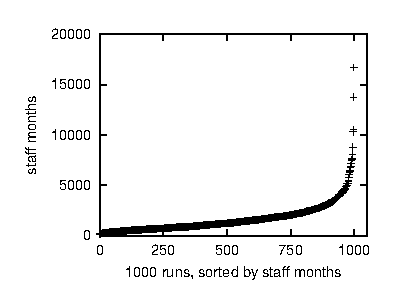
\includegraphics[width=3.2in]{coc1Kruns.eps}
\end{center}
\caption{Sample output.}\label{fig:coc1Kruns}
\end{figure}

% %\input{lurch0}
% %\input{memo1}
% %\input{lurch1}
% %\input{omolib}
% %\input{lurch2}
% %\input{fib}
\section{ Bugs }
None known but many suspected.



\theend
\end{document}

